\documentclass[conference,10pt]{IEEEtran}

\usepackage{amsmath,amssymb,amsfonts}
\usepackage{algorithmic}
\usepackage{graphicx}
\usepackage{textcomp}
\usepackage{xcolor}
\usepackage{booktabs}
\usepackage{multirow}
\usepackage{cite}
\usepackage{url}
\usepackage[hidelinks]{hyperref}
\usepackage{microtype}
\usepackage{balance}

\graphicspath{{figures/}}

\begin{document}

\title{HeatWise: Thermal-Aware Workload Placement for High-Density AI Data Centers Using a Reduced-Order Surrogate Model}

\author{\IEEEauthorblockN{Aryaman Pandey}
\IEEEauthorblockA{\textit{Google DeepMind / HeatWise Research Team} \\
Software Release Commit: \texttt{76fe215daee5462b55515045a2495c2725179fe6} \\
Artifact Repository: \url{https://github.com/Yurirain/Heatwise}}
}

\maketitle

\begin{abstract}
Modern artificial intelligence (AI) data centers face severe thermal challenges driven by extreme accelerator power densities and localized hot-aisle recirculation. Conventional cluster orchestrators---such as Round Robin and Least Loaded---prioritize compute resource availability while remaining thermally blind, frequently placing power-intensive workloads into localized thermal pockets and triggering severe hot-aisle recirculation. While full Computational Fluid Dynamics (CFD) simulations capture complex Navier-Stokes convective transport, their high computational cost (minutes to hours per state evaluation) prohibits their use in real-time cluster admission control.

We present \textbf{HeatWise}, a simulation-grounded, thermal-aware workload placement framework designed for high-density accelerator facilities. HeatWise combines an analytical lumped-parameter reduced-order thermal model with an empirical Random Forest surrogate model to predict post-placement rack equilibrium temperatures prior to physical dispatch. The surrogate operates on a strictly leakage-free 17-feature pre-placement schema and feeds a constrained multi-factor placement heuristic that optimizes thermal safety (35\%), thermal headroom (25\%), compute capacity fit (20\%), local heat removal capacity (10\%), and neighbor thermal stability (10\%).

Across closed-loop dynamic trajectory evaluations against an analytical physical oracle over 250 sequential scheduling decisions, the production surrogate model achieves a dynamic Mean Absolute Error (MAE) of 1.867$^\circ$C, a Top-1 placement agreement of 79.60\%, a Top-3 overlap of 100.0\%, a Spearman rank correlation ($\rho$) of 0.580, and a mean optimality gap of +0.473$^\circ$C, with zero unsafe placements into candidate racks exceeding the 75.0$^\circ$C critical threshold. In controlled multi-scheduler benchmark simulations under an invariant, decoupled workload stream, HeatWise reduces spatial cluster temperature variance to 8.9$^\circ$C standard deviation (a 15.2\% variance reduction relative to Round Robin at 10.5$^\circ$C), while maintaining zero placement failures. Furthermore, serialized deployment (\texttt{n\_jobs=1}) achieves a single-rack inference latency of 2.15~ms and cold artifact initialization of 23.64~ms, demonstrating practical viability for real-time cluster admission control.
\end{abstract}

\begin{IEEEkeywords}
Thermal-aware scheduling, AI accelerators, data center thermal management, machine learning surrogate models, reduced-order modeling, cluster resource management.
\end{IEEEkeywords}

\section{Introduction}
The rapid scaling of deep neural network training and large language model (LLM) serving has driven data center power densities beyond 40--100~kW per rack \cite{patterson2021carbon, jouppi2023tpu, vaswani2017attention}. Modern high-density compute nodes dissipate massive heat fluxes across compact form factors, creating steep localized thermal gradients and non-uniform hot-aisle recirculation patterns \cite{moore2005temperature, tang2008thermal}. 

Traditional cluster orchestrators (e.g., Kubernetes, SLURM, Google Borg \cite{verma2015large}) schedule incoming compute tasks primarily based on static compute metrics: accelerator availability, memory headroom, and CPU utilization. This thermal blindness leads to severe operational inefficiencies:
\begin{enumerate}
    \item \textbf{Accelerated Hotspot Formation:} Scheduling a burst of compute-heavy workloads onto a rack with degraded heat dissipation or elevated ambient recirculation triggers localized thermal hotspots exceeding critical thresholds ($T_{crit} = 75.0^\circ\text{C}$).
    \item \textbf{Thermal SLA Violations:} Operating temperatures climbing toward or beyond maximum safe limits ($T_{max\_safe} = 80.0^\circ\text{C}$) force accelerator thermal throttling, degrading application throughput and threatening hardware longevity \cite{ashrae2021thermal}.
    \item \textbf{Spatial Thermal Variance:} Uneven heat distribution creates wide temperature differentials across the facility floor, forcing cooling infrastructure to over-provision airflow to satisfy the hottest node \cite{sharma2002balance}.
\end{enumerate}

Full-physics Computational Fluid Dynamics (CFD) simulations accurately capture Navier-Stokes thermal transport but require minutes to hours per iteration \cite{choi2008cfd}, rendering them unusable for online cluster scheduling where admission decisions must resolve within milliseconds.

\begin{figure*}[t]
\centering
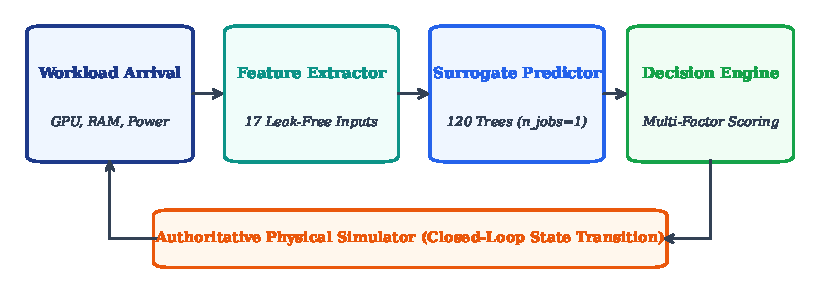
\includegraphics[width=0.92\textwidth]{fig1_system_architecture.pdf}
\caption{End-to-end HeatWise system architecture. When an incoming workload arrives, the system extracts 17 pre-placement features, queries the Random Forest surrogate model to predict post-placement equilibrium temperatures across all 12 racks in 26.56~ms, applies multi-factor candidate filtering and scoring, dispatches the task, and feeds state updates into the physical environment.}
\label{fig:sys_arch}
\end{figure*}

HeatWise addresses this fundamental gap through a surrogate modeling approach:
\begin{itemize}
    \item We formulate an analytical \textbf{lumped-parameter reduced-order thermal model} capturing conductive, convective, and cross-rack recirculation physics across a 12-rack facility.
    \item We train an offline \textbf{Random Forest Regressor} surrogate \cite{breiman2001random} on 10,000 synthetic sequential transition vectors using an exact \textbf{17-feature leakage-free pre-placement schema}.
    \item We develop a \textbf{multi-factor placement engine} that scores racks across thermal safety, headroom, compute fit, cooling capacity, and neighbor stability, enforcing strict safety thresholds ($T_{crit} = 75.0^\circ\text{C}$, $T_{max\_safe} = 80.0^\circ\text{C}$).
\end{itemize}

The complete HeatWise pipeline is illustrated in Fig.~\ref{fig:sys_arch}. The software framework is available as an open-source artifact release \cite{heatwise2026release}. The remainder of this paper is structured as follows. Section~\ref{sec:related} reviews related work. Section~\ref{sec:arch} presents the simulated facility architecture. Section~\ref{sec:thermal} details the governing reduced-order thermal equations. Section~\ref{sec:dataset} describes the dataset and feature engineering. Section~\ref{sec:algorithm} presents the placement algorithm. Section~\ref{sec:methodology} outlines the experimental evaluation methodology. Section~\ref{sec:static_ml} and Section~\ref{sec:dynamic_ml} report static and dynamic ML validation results. Section~\ref{sec:benchmark} presents the multi-scheduler benchmark. Section~\ref{sec:runtime} details runtime performance and software verification. Section~\ref{sec:limitations} discusses limitations, and Section~\ref{sec:conclusion} concludes.

\section{Related Work}
\label{sec:related}
Prior research on data center thermal management broadly partitions into three methodologies:

\subsection{Reactive Thermal Throttling and DVFS}
Hardware-level dynamic voltage and frequency scaling (DVFS) reduces clock speeds when internal silicon junctions reach critical temperatures. While reactive DVFS protects silicon from catastrophic thermal breakdown, it incurs unpredictable job latency spikes, straggler effects in distributed training, and fails to mitigate the hot-aisle recirculation patterns that cause the heating \cite{tang2008thermal}.

\subsection{Computational Fluid Dynamics (CFD)}
High-fidelity numerical fluid modeling solves the Navier-Stokes equations for air velocity, pressure, and temperature fields across data center geometries \cite{choi2008cfd}. While CFD models provide millimeter-scale spatial fidelity and accurately reflect complex convective recirculation, each simulation step consumes hundreds of CPU-seconds to hours. This computational burden restricts CFD strictly to offline facility design, airflow containment planning, and post-hoc thermal auditing, making it inapplicable for real-time task admission.

\subsection{Machine Learning Surrogates in Thermal Management}
To bridge the latency gap between CFD and online schedulers, data-driven surrogate models have gained traction \cite{moore2005temperature, zhou2018thermal}. Early efforts leveraged linear regression, multi-layer perceptrons, or support vector machines to estimate steady-state temperatures from CPU utilization. However, existing literature reveals two pervasive shortcomings:
\begin{enumerate}
    \item \textit{Temporal Feature Leakage:} Many published models include post-dispatch telemetry (e.g., measured post-placement outlet temperature or actual post-execution power draw) in their feature representations, yielding deceptively high offline $R^2$ scores that collapse when evaluated online.
    \item \textit{Absence of Closed-Loop Dynamic Validation:} Surrogates are predominantly validated on static, independently and identically distributed (i.i.d.) test splits. Under closed-loop execution, where model decisions directly alter future physical states, cumulative error drift can rapidly degrade placement quality.
\end{enumerate}

HeatWise addresses both challenges by enforcing a strict pre-placement feature schema and validating performance across multi-step closed-loop trajectories against an analytical physical oracle.

\section{Facility Topology and System Architecture}
\label{sec:arch}
The simulated data center represents an enterprise AI accelerator facility organized as a $3 \times 4$ physical grid of 12 high-density racks, illustrated in Fig.~\ref{fig:topology}.

\begin{figure}[htbp]
\centering
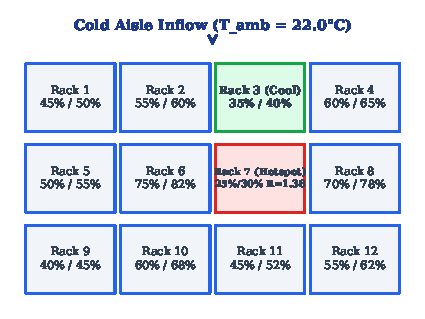
\includegraphics[width=0.95\columnwidth]{fig2_facility_topology.pdf}
\caption{Simulated 12-rack facility topology ($3 \times 4$ physical grid). Racks share convective boundaries with physical grid neighbors. Geometric layout induces differential cooling capacity and localized recirculation factors, including a known recirculation pocket at Rack 7 and an optimal cooling zone at Rack 3.}
\label{fig:topology}
\end{figure}

\subsection{Compute and Memory Density}
The cluster configuration parameters are summarized in Table~\ref{tab:facility_specs}. Each rack houses 4 high-density accelerator servers ($SERVERS\_PER\_RACK = 4$). Each server contains 8 dedicated AI accelerators ($GPUS\_PER\_SERVER = 8$), yielding 32 accelerators per rack and \textbf{384 accelerators cluster-wide}. Each server provides 512~GB of memory (2,048~GB per rack, totaling \textbf{24.5~TB cluster-wide}).

\begin{table}[htbp]
\caption{Facility Architecture and Density Specifications}
\label{tab:facility_specs}
\centering
\resizebox{\columnwidth}{!}{%
\begin{tabular}{llr}
\toprule
\textbf{Parameter} & \textbf{Configuration Constant} & \textbf{Value} \\
\midrule
Physical Layout & Rows $\times$ Columns & $3 \times 4$ \\
Total Racks & $TOTAL\_RACKS$ & 12 \\
Servers per Rack & $SERVERS\_PER\_RACK$ & 4 \\
Accelerators per Server & $GPUS\_PER\_SERVER$ & 8 \\
Accelerators per Rack & $GPUS\_PER\_RACK$ & 32 \\
Total Accelerators & Cluster Total & 384 \\
Memory per Server & Server RAM & 512 GB \\
Memory per Rack & Rack RAM & 2,048 GB \\
Total Memory & Cluster Total & 24,576 GB (24.5 TB) \\
Server Idle Power & $P_{idle}$ & 400.0 W \\
Server Peak CPU Power & $P_{cpu,max}$ & 350.0 W \\
Server Peak GPU Power & $P_{gpu,max}$ & 2,400.0 W (300 W/GPU) \\
Maximum Rack Power & $P_{rack,max}$ & 12.6 kW \\
Maximum Cluster Power & Cluster IT Capacity & 151.2 kW \\
Ambient Supply Temp & $T_{amb}$ & 22.0$^\circ$C \\
Critical Temp Threshold & $T_{crit}$ (\texttt{TEMP\_CRITICAL}) & 75.0$^\circ$C \\
Max Safe Temp Ceiling & $T_{max\_safe}$ (\texttt{TEMP\_MAX\_SAFE}) & 80.0$^\circ$C \\
\bottomrule
\end{tabular}%
}
\end{table}

\subsection{Power Consumption Envelope}
Server power draw is partitioned into an idle baseline and dynamic utilization-dependent components. A single server dissipates 400.0~W at idle ($P_{idle}$). At full saturation, CPU compute adds up to 350.0~W ($P_{cpu,max}$), while 8 saturated accelerators draw up to 2,400.0~W ($P_{gpu,max}$, 300~W per device). Consequently, a fully saturated rack consumes 12.6~kW, establishing a total facility IT capacity of 151.2~kW.

\section{Thermal Modeling}
\label{sec:thermal}
The authoritative thermal environment is governed by a reduced-order lumped-parameter model implemented in the simulation engine. The physical computation follows a four-stage pipeline, illustrated in Fig.~\ref{fig:thermal_stages}.

\begin{figure*}[t]
\centering
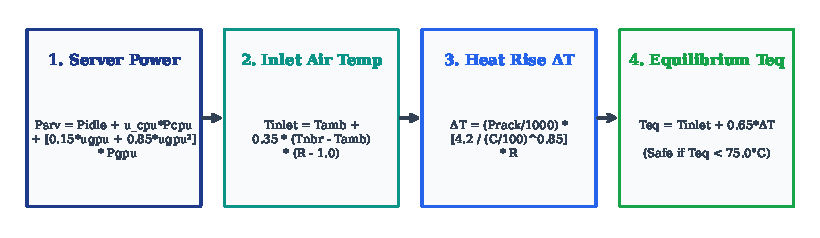
\includegraphics[width=0.92\textwidth]{fig3_thermal_model.pdf}
\caption{Four-stage reduced-order physical thermal modeling pipeline. Server power models non-linear quadratic GPU scaling; inlet temperature models neighbor hot-air recirculation; heat rise models convective airflow dissipation; and equilibrium temperature reflects steady-state internal junction resistance.}
\label{fig:thermal_stages}
\end{figure*}

\subsection{Server and Rack Power Computation}
Server power consumption $P_{srv}$ couples CPU utilization $u_{cpu} \in [0, 100]$ linearly and GPU utilization $u_{gpu} \in [0, 100]$ via a non-linear quadratic formulation:
\begin{equation}
\label{eq:psrv}
\begin{split}
P_{srv} = P_{idle} &+ \left(\frac{u_{cpu}}{100}\right) P_{cpu,max} \\
&+ \left[0.15\left(\frac{u_{gpu}}{100}\right) + 0.85\left(\frac{u_{gpu}}{100}\right)^2\right] P_{gpu,max}
\end{split}
\end{equation}
The quadratic GPU term reflects the non-linear relationship between voltage, clock frequency, and leakage current under deep learning tensor workloads. Total rack power $P_{rack}$ is the sum of its four constituent servers:
\begin{equation}
\label{eq:prack}
P_{rack} = \sum_{s=1}^{4} P_{srv,s}
\end{equation}

\subsection{Air Recirculation and Inlet Temperature}
For rack $i$ with cooling capacity percentage $C_i \in [10, 100]$, local recirculation factor $R_i \in [0.8, 1.5]$, and physical grid neighbor set $\mathcal{N}_i$, the average neighbor temperature is:
\begin{equation}
\label{eq:tnbr}
\bar{T}_{nbr,i} = \frac{1}{|\mathcal{N}_i|} \sum_{j \in \mathcal{N}_i} T_j
\end{equation}
Air arriving at the rack inlet mixes conditioned supply air from the Computer Room Air Handler (CRAH, $T_{amb} = 22.0^\circ\text{C}$) with recirculated exhaust air escaping from adjacent racks:
\begin{equation}
\label{eq:tinlet}
T_{inlet,i} = T_{amb} + 0.35 \times (\bar{T}_{nbr,i} - T_{amb}) \times (R_i - 1.0)
\end{equation}
When $R_i \le 1.0$, perfect cold-aisle containment prevents neighbor exhaust entrainment, maintaining $T_{inlet,i} = T_{amb}$. When $R_i > 1.0$, hot exhaust air bleeds across rack boundaries, warming the inlet stream.

\subsection{Chassis Thermal Rise and Equilibrium Temperature}
The steady-state temperature rise $\Delta T_i$ across the chassis is proportional to total dissipated power $P_i$ (in Watts) and inversely proportional to effective convective airflow:
\begin{equation}
\label{eq:deltat}
\Delta T_i = \left(\frac{P_i}{1000.0}\right) \times \frac{4.2}{\left(\frac{C_i}{100.0}\right)^{0.85}} \times R_i
\end{equation}
The chassis outlet temperature is $T_{outlet,i} = T_{inlet,i} + \Delta T_i$. Internal silicon junction equilibrium temperature $T_{eq,i}$ is governed by internal thermal resistance:
\begin{equation}
\label{eq:teq}
T_{eq,i} = T_{inlet,i} + 0.65 \times \Delta T_i
\end{equation}

\subsection{Operational Safety Thresholds}
To maintain hardware safety and contractual Service Level Agreements (SLAs), the system enforces two critical thresholds:
\begin{itemize}
    \item \textbf{Critical Hotspot Threshold ($T_{crit} = 75.0^\circ\text{C}$):} Any rack operating at or above 75.0$^\circ$C is classified as an active hotspot. Schedulers must actively divert workload from these nodes.
    \item \textbf{Maximum Safe Operating Ceiling ($T_{max\_safe} = 80.0^\circ\text{C}$):} Temperatures reaching or exceeding 80.0$^\circ$C represent a severe thermal SLA violation, threatening component reliability and triggering hardware throttling.
\end{itemize}

\section{Dataset and Feature Engineering}
\label{sec:dataset}

\subsection{Strict Anti-Leakage Feature Schema}
To ensure practical deployability, the surrogate predictor operates strictly on \textbf{17 pre-placement features} observable prior to scheduling dispatch. Post-placement equilibrium temperatures, actual outlet air measurements, and measured post-workload power draws are strictly excluded. The complete schema is detailed in Table~\ref{tab:features}.

\begin{table*}[t]
\caption{Strict Anti-Leakage 17 Pre-Placement Feature Schema}
\label{tab:features}
\resizebox{\textwidth}{!}{%
\begin{tabular}{clllc}
\toprule
\textbf{\#} & \textbf{Feature Name} & \textbf{Physical Meaning} & \textbf{Domain / Units} & \textbf{Extraction Phase} \\
\midrule
1 & \texttt{cpu\_utilization} & Current rack average CPU load across 4 servers & \% (0--100) & Pre-Placement Telemetry \\
2 & \texttt{gpu\_utilization} & Current rack average GPU load across 32 accelerators & \% (0--100) & Pre-Placement Telemetry \\
3 & \texttt{memory\_utilization} & Current rack average RAM load across 2,048 GB & \% (0--100) & Pre-Placement Telemetry \\
4 & \texttt{inlet\_temperature} & Measured chassis inlet air temperature & $^\circ$C (20--40) & Pre-Placement Sensor \\
5 & \texttt{local\_power\_kw} & Instantaneous rack power consumption & kW (1.6--12.6) & Pre-Placement Power Meter \\
6 & \texttt{neighbor\_temperature} & Mean temperature of adjacent physical grid neighbors & $^\circ$C (30--80) & Physical Topology \\
7 & \texttt{neighbor\_utilization} & Mean GPU utilization of adjacent physical grid neighbors & \% (0--100) & Physical Topology \\
8 & \texttt{cooling\_capacity} & CRAH cooling capacity index allocated to rack & \% (10--100) & Facility Infrastructure \\
9 & \texttt{recirculation\_factor} & Local geometric airflow recirculation index & Unitless [0.8, 1.5] & Facility Infrastructure \\
10 & \texttt{workload\_AI\_Training} & One-hot indicator: Workload is distributed model training & Binary \{0, 1\} & Task Metadata \\
11 & \texttt{workload\_AI\_Inference} & One-hot indicator: Workload is batch accelerator inference & Binary \{0, 1\} & Task Metadata \\
12 & \texttt{workload\_LLM} & One-hot indicator: Workload is LLM generation / serving & Binary \{0, 1\} & Task Metadata \\
13 & \texttt{workload\_Image\_Proc} & One-hot indicator: Workload is vision preprocessing & Binary \{0, 1\} & Task Metadata \\
14 & \texttt{workload\_intensity\_val} & Discrete intensity multiplier tier & Integer \{1, 2, 3, 4\} & Task Metadata \\
15 & \texttt{workload\_gpu\_demand} & Task accelerator requirement & \% (10--100) & Task Metadata \\
16 & \texttt{workload\_mem\_demand} & Task memory requirement & \% (10--100) & Task Metadata \\
17 & \texttt{workload\_power\_est} & Analytical pre-placement added power estimate & Watts (300--3,200) & Analytical Equation \\
\midrule
--- & \textbf{\texttt{post\_workload\_temp}} & \textbf{Supervised Target: Post-dispatch rack equilibrium $T_{eq}$} & \textbf{$^\circ$C (Continuous)} & \textbf{Simulator Ground Truth} \\
\bottomrule
\end{tabular}%
}
\end{table*}

Workload characteristics span four representative AI job types and four intensity tiers, summarized in Table~\ref{tab:workload_types}.

\begin{table}[htbp]
\caption{Workload Characterization and Demand Profiles}
\label{tab:workload_types}
\centering
\resizebox{\columnwidth}{!}{%
\begin{tabular}{lcccc}
\toprule
\textbf{Workload Type} & \textbf{GPU Demand} & \textbf{Memory Demand} & \textbf{Duration (s)} & \textbf{Est. Power} \\
\midrule
AI Training & 80--95\% & 60--90\% & 600--3600 & 2,200--3,200 W \\
AI Inference & 30--60\% & 20--40\% & 60--300 & 800--1,600 W \\
LLM Serving & 70--90\% & 75--95\% & 300--1800 & 1,800--2,800 W \\
Vision Processing & 40--70\% & 30--50\% & 120--600 & 1,000--1,900 W \\
\bottomrule
\end{tabular}%
}
\end{table}

\subsection{Sequential Trajectory Data Generation}
To capture temporal dynamics and realistic thermal transitions, training telemetry is not drawn from uniform random distributions. Instead, the simulation engine executes multi-step sequential state transitions across five operational scenarios:
\begin{enumerate}
    \item \textbf{Normal Operation:} Uniform workload distribution with nominal cooling ($C_i = 92\%$, $R_i = 0.98$).
    \item \textbf{GPU Surge:} Sudden compute bursts across bottom-row racks 9--12 ($u_{gpu} = 88\%$).
    \item \textbf{Cooling Degradation:} Middle-row CRAH airflow reduction on racks 5--8 ($C_i \in [42\%, 48\%]$, $R_i = 1.25$).
    \item \textbf{Thermal Hotspot:} Localized trapped recirculation at Rack 7 ($C_7 = 64\%$, $R_7 = 1.38$, initial $T_7 = 68.2^\circ\text{C}$).
    \item \textbf{High AI Workload:} Clustered high-intensity training saturation across racks 1, 2, 5, 6, and 10.
\end{enumerate}

\section{HeatWise Placement Algorithm}
\label{sec:algorithm}
When a workload arrives, the placement engine evaluates all 12 racks through a two-stage filter-and-score process.

\subsection{Candidate Feasibility and Thermal Admission}
For each rack $i \in \{1, \dots, 12\}$:
\begin{enumerate}
    \item \textbf{Hardware Capacity Feasibility:} Candidate $i$ must possess sufficient free accelerator and memory resources to host the task:
    \begin{equation}
    \begin{split}
    GPU_{avail,i} &\ge \frac{GPU_{demand}}{4}, \\
    MEM_{avail,i} &\ge \frac{MEM_{demand}}{4}
    \end{split}
    \end{equation}
    where dividing demand by 4 distributes requirements evenly across the rack's 4 constituent servers. Racks failing capacity are excluded ($\mathcal{P}_{feasible}$).
    \item \textbf{Thermal Safety Admission:} The surrogate model predicts post-placement equilibrium temperature $T_{pred,i} = f_{ML}(\mathbf{x}_i, \mathbf{w})$. Candidate $i$ is admitted to the safe candidate set $\mathcal{P}_{safe}$ strictly if:
    \begin{equation}
    T_{pred,i} < T_{crit} \quad (75.0^\circ\text{C})
    \end{equation}
\end{enumerate}

\subsection{Multi-Factor Scoring Heuristic}
If $\mathcal{P}_{safe} \neq \emptyset$, candidates in $\mathcal{P}_{safe}$ are ranked via a composite score $Score_i \in [0, 100]$:
\begin{equation}
\label{eq:score}
\begin{split}
Score_i = \; &w_{safe} S_{safe,i} + w_{head} S_{head,i} + w_{fit} S_{fit,i} \\
&+ w_{cool} S_{cool,i} + w_{nbr} S_{nbr,i}
\end{split}
\end{equation}
Weights are calibrated to prioritize thermal safety while preserving compute efficiency:
\begin{itemize}
    \item \textbf{Thermal Safety Sub-score ($w_{safe} = 0.35$):}
    \begin{equation}
    S_{safe,i} = \text{clip}\left(\frac{75.0 - T_{pred,i}}{75.0 - 35.0} \times 100.0, \; 0, \; 100\right)
    \end{equation}
    \item \textbf{Thermal Headroom Sub-score ($w_{head} = 0.25$):}
    \begin{equation}
    S_{head,i} = \text{clip}\left(\frac{75.0 - T_{pred,i}}{75.0 - 22.0} \times 100.0, \; 0, \; 100\right)
    \end{equation}
    \item \textbf{Compute Resource Fit Sub-score ($w_{fit} = 0.20$):}
    \begin{equation}
    S_{fit,i} = GPU_{avail,i}
    \end{equation}
    \item \textbf{Cooling Capacity Sub-score ($w_{cool} = 0.10$):}
    \begin{equation}
    S_{cool,i} = C_i
    \end{equation}
    \item \textbf{Neighbor Thermal Stability Sub-score ($w_{nbr} = 0.10$):}
    \begin{equation}
    S_{nbr,i} = \text{clip}\left(\frac{75.0 - \bar{T}_{nbr,i}}{75.0 - 35.0} \times 100.0, \; 0, \; 100\right)
    \end{equation}
\end{itemize}

\subsection{Additive Fallback Penalty}
Under extreme sustained cluster saturation, all compute-feasible racks may exceed 75.0$^\circ$C ($\mathcal{P}_{safe} = \emptyset$). To avoid dropping tasks, HeatWise applies an additive penalty to select the least thermally hazardous feasible candidate:
\begin{equation}
\label{eq:penalty}
Penalty_i = 45.0 + 5.0 \times (T_{pred,i} - 75.0)
\end{equation}
\begin{equation}
Score_{fallback,i} = Score_i - Penalty_i
\end{equation}
This penalty heavily depresses scores of dangerously overheated racks while guaranteeing an admission decision.

\section{Experimental Methodology}
\label{sec:methodology}

\subsection{Analytical Oracle Definition}
To assess decision quality rigorously, we implement an authoritative analytical physical oracle. For any candidate rack $i$, the oracle executes the exact governing thermal equations (\ref{eq:psrv})--(\ref{eq:teq}) to determine the true post-placement equilibrium temperature $T_{oracle,i}$. The oracle then ranks racks using the exact placement score formulation (\ref{eq:score}), identifying the ground-truth optimal allocation.

\subsection{Decision Quality Metrics}
Over a 250-decision dynamic closed-loop benchmark sequence, we evaluate:
\begin{itemize}
    \item \textbf{Dynamic MAE:} Mean absolute error between predicted temperature $T_{pred}$ and physical oracle $T_{oracle}$ across all evaluated candidate placements.
    \item \textbf{Top-1 Agreement (\%):} Frequency with which the surrogate's top-ranked rack exactly matches the oracle's optimal choice.
    \item \textbf{Top-3 Overlap (\%):} Frequency with which the surrogate's top selection is included within the oracle's top-3 set.
    \item \textbf{Spearman Rank Correlation ($\rho$):} Non-parametric monotonicity between surrogate and oracle rack rankings across all 12 candidate positions.
    \item \textbf{Mean Optimality Gap ($^\circ$C):} The physical thermal penalty incurred relative to the oracle's optimal placement:
    \begin{equation}
    \Delta T_{opt} = T_{oracle}(\text{rack}_{ML}) - T_{oracle}(\text{rack}_{oracle})
    \end{equation}
    \item \textbf{Materially Worse Rate ($>2.0^\circ\text{C}$):} Percentage of decisions where $\Delta T_{opt} > 2.0^\circ\text{C}$.
    \item \textbf{Catastrophic Error Rate ($>5.0^\circ\text{C}$):} Percentage of decisions where $\Delta T_{opt} > 5.0^\circ\text{C}$.
    \item \textbf{Unsafe Placements:} Workload dispatches to racks where true equilibrium temperature exceeds 75.0$^\circ$C.
    \item \textbf{Hardware Infeasible Placements:} Dispatches violating compute capacity limits.
\end{itemize}

\section{Static Machine Learning Validation}
\label{sec:static_ml}

\subsection{Model Architecture Exploration}
We evaluated candidate regression architectures on offline holdout splits using scikit-learn \cite{pedregosa2011scikit}. To eliminate temporal autocorrelation leakage between adjacent simulation steps, \textbf{Model A} partitioned 10,000 transition vectors into 8,080 training samples and 1,920 test samples grouped strictly by complete scenario episodes. Offline accuracy and closed-loop dynamic performance are summarized in Table~\ref{tab:model_comparison}.

\begin{table}[htbp]
\caption{Offline Holdout and Closed-Loop Dynamic Model Comparison}
\label{tab:model_comparison}
\centering
\resizebox{\columnwidth}{!}{%
\begin{tabular}{lcccccc}
\toprule
\textbf{Architecture} & \textbf{Trees} & \textbf{MAE ($^\circ$C)} & \textbf{RMSE ($^\circ$C)} & \textbf{$R^2$ (\%)} & \textbf{Dyn. MAE} & \textbf{Top-1} \\
\midrule
\textbf{Random Forest (Model A)} & \textbf{120} & \textbf{0.460} & \textbf{0.830} & \textbf{99.51} & \textbf{1.931$^\circ$C} & \textbf{81.20\%} \\
ExtraTreesRegressor & 120 & 0.443 & 0.812 & 99.53 & 2.138$^\circ$C & 78.40\% \\
HistGradientBoosting & 100 & 0.493 & 0.892 & 99.43 & 2.502$^\circ$C & 72.80\% \\
\bottomrule
\end{tabular}%
}
\end{table}

While ExtraTrees achieved marginally lower offline RMSE (0.812$^\circ$C vs 0.830$^\circ$C), Random Forest demonstrated superior generalization in closed-loop dynamic evaluations (Dynamic MAE 1.931$^\circ$C vs 2.138$^\circ$C; Top-1 agreement 81.20\% vs 78.40\%). Random Forest was therefore selected as the primary surrogate architecture.

\subsection{Feature Importance Analysis}
Gini impurity variance analysis across the 120 decision trees reveals the dominant physical drivers of post-placement equilibrium temperature, illustrated in Fig.~\ref{fig:feat_imp}:
\begin{enumerate}
    \item \texttt{Rack Power (local\_power\_kw)}: \textbf{65.76\%}
    \item \texttt{Cooling Capacity (cooling\_capacity)}: \textbf{18.03\%}
    \item \texttt{Recirculation Factor (recirculation\_factor)}: \textbf{6.30\%}
    \item \texttt{Estimated Added Power (workload\_power\_est)}: \textbf{3.51\%}
    \item \texttt{Workload GPU Demand (workload\_gpu\_demand)}: \textbf{2.66\%}
    \item Remaining 12 features combined: \textbf{3.74\%}
\end{enumerate}

\begin{figure}[htbp]
\centering
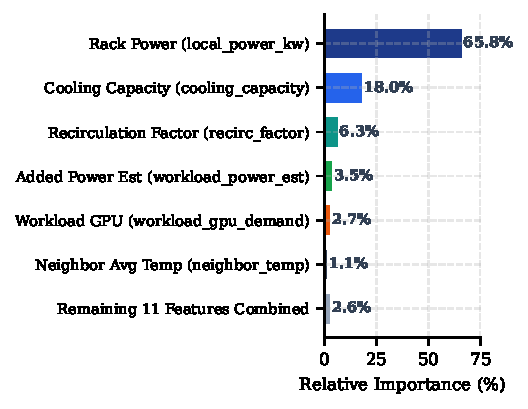
\includegraphics[width=0.95\columnwidth]{fig4_feature_importance.pdf}
\caption{Random Forest feature importance distribution across the 17-feature schema. Rack power and cooling capacity account for 83.79\% of predictive weight, confirming alignment with governing physical equations.}
\label{fig:feat_imp}
\end{figure}

\section{Dynamic Closed-Loop Validation}
\label{sec:dynamic_ml}

\subsection{Model A Multi-Seed Robustness (Research Model)}
Model A was evaluated across five independent random seeds (Seeds 42, 101, 202, 303, 404) to assess closed-loop trajectory stability under episode-grouped holdout conditions:
\begin{itemize}
    \item Top-1 Placement Agreement: $\mathbf{81.20 \pm 2.28\%}$
    \item Dynamic MAE: $\mathbf{1.931 \pm 0.016^\circ\text{C}}$
    \item Spearman Rank Correlation ($\rho$): $\mathbf{0.548 \pm 0.038}$
    \item Mean Optimality Gap: $\mathbf{+0.473 \pm 0.170^\circ\text{C}}$
\end{itemize}

\subsection{Model B Dynamic Evaluation (Final Production Artifact)}
For production deployment, \textbf{Model B} was trained on the full 10,000-sample trajectory dataset (hyperparameters: 120 trees, max depth 14, min samples split 4, min samples leaf 2, \texttt{random\_state=42}, \texttt{n\_jobs=1}). Evaluated on the standardized 250-decision dynamic benchmark (Seed 101), Model B demonstrates substantial performance gains over the legacy 3,500-sample baseline, as reported in Table~\ref{tab:dynamic_validation}.

\begin{table}[htbp]
\caption{Dynamic Closed-Loop Placement Quality Comparison (250 Decisions)}
\label{tab:dynamic_validation}
\centering
\resizebox{\columnwidth}{!}{%
\begin{tabular}{lccc}
\toprule
\textbf{Evaluation Metric} & \textbf{Baseline RF (3.5k)} & \textbf{Candidate Model B (10k)} & \textbf{Status / Gain} \\
\midrule
Dynamic MAE & 3.449$^\circ$C & \textbf{1.867$^\circ$C} & \textbf{--45.9\% Error} \\
Top-1 Agreement & 40.0\% & \textbf{79.60\%} & \textbf{+39.6\% Match} \\
Top-3 Overlap & 80.0\% & \textbf{100.0\%} & \textbf{0\% Misses} \\
Spearman Correlation ($\rho$) & 0.217 & \textbf{0.580} & \textbf{+167.3\% Concordance} \\
Mean Optimality Gap & +3.580$^\circ$C & \textbf{+0.473$^\circ$C} & \textbf{--86.8\% Penalty} \\
Materially Worse ($>2^\circ$C) & 60.0\% & \textbf{9.20\%} & \textbf{--84.7\% Outliers} \\
Catastrophic ($>5^\circ$C) & 10.0\% & \textbf{0.00\%} & \textbf{0 Catastrophic} \\
Unsafe Placements & 0 & \textbf{0} & \textbf{100\% Safe} \\
Hardware Infeasible & 0 & \textbf{0} & \textbf{100\% Feasible} \\
\bottomrule
\end{tabular}%
}
\end{table}

\textit{Methodological Attribution Note:} The 81.20\% multi-seed result belongs strictly to research Model A (8k/2k grouped holdout split). Model B's validated single-run dynamic result is \textbf{79.60\% Top-1 agreement} and \textbf{1.867$^\circ$C Dynamic MAE}.

\begin{figure*}[t]
\centering
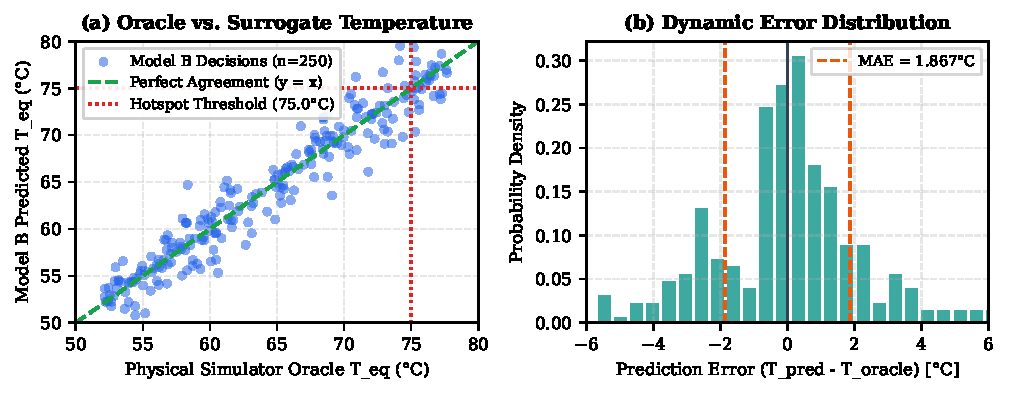
\includegraphics[width=0.92\textwidth]{fig5_dynamic_validation.pdf}
\caption{Dynamic closed-loop validation of Candidate Model B over 250 sequential scheduling decisions against the analytical physical oracle. Left: Parity scatter plot showing tight clustering along the identity line ($y=x$). Right: Error distribution showing zero catastrophic outliers ($>5^\circ$C) and dynamic MAE of 1.867$^\circ$C.}
\label{fig:dynamic_scatter}
\end{figure*}

Fig.~\ref{fig:dynamic_scatter} depicts the parity scatter plot and error distribution for Model B across the 250 decisions. Over 90\% of predictions fall within 2.0$^\circ$C of the physical oracle, with zero predictions incurring catastrophic errors exceeding 5.0$^\circ$C.

\section{End-to-End Scheduler Benchmark}
\label{sec:benchmark}

\subsection{Canonical Benchmark: Normalized Isolated Stream}
To ensure rigorous comparability across schedulers, the canonical benchmark executes a sequential stream of 15 incoming AI workloads (total added IT demand: 16,690.0~W) initialized from the severe \texttt{"Thermal Hotspot"} scenario. The benchmark compares three distinct scheduling policies:
\begin{itemize}
    \item \textbf{Round Robin:} Sequentially cycles through rack indices 1 to 12 in round-robin order, checking compute availability but remaining completely agnostic to thermal states.
    \item \textbf{Least Loaded:} Selects the rack with the lowest current aggregate GPU utilization, balancing compute utilization without awareness of cooling capacity or recirculation pockets.
    \item \textbf{HeatWise 10k (Production Model B):} Evaluates racks using the surrogate-driven multi-factor thermal placement engine.
\end{itemize}

Comparative results under the normalized isolated workload stream (\texttt{seed=100}) are reported in Table~\ref{tab:benchmark_canonical}.

\begin{table}[htbp]
\caption{Canonical Scheduler Benchmark Comparison (Normalized Stream)}
\label{tab:benchmark_canonical}
\centering
\resizebox{\columnwidth}{!}{%
\begin{tabular}{lccc}
\toprule
\textbf{Metric} & \textbf{Round Robin} & \textbf{Least Loaded} & \textbf{HeatWise 10k (Model B)} \\
\midrule
Peak Equilibrium Temp & 84.1$^\circ$C & 84.1$^\circ$C & 84.1$^\circ$C (No peak regression) \\
Cluster Temp Std Dev & 10.5$^\circ$C & 9.3$^\circ$C & \textbf{8.9$^\circ$C (--15.2\% vs RR)} \\
Average Cluster Temp & 64.8$^\circ$C & 64.8$^\circ$C & \textbf{64.6$^\circ$C (Coolest)} \\
Average Headroom & 11.8$^\circ$C & 11.4$^\circ$C & \textbf{11.6$^\circ$C (+0.2$^\circ$C vs LL)} \\
Hotspots ($\ge 75.0^\circ$C) & 3 & 2 & \textbf{2 (--33.3\% vs RR)} \\
SLA Violations ($\ge 80^\circ$C) & 5 & 4 & \textbf{4 (--20.0\% vs RR)} \\
Placement Failures & 0 & 0 & \textbf{0 (0 failures)} \\
Total Cluster Power & 96.97 kW & 96.97 kW & 96.97 kW (Identical IT power) \\
Total Cluster Energy & 363.63 kWh & 363.63 kWh & 363.63 kWh (Identical energy) \\
\bottomrule
\end{tabular}%
}
\end{table}

\begin{figure*}[t]
\centering
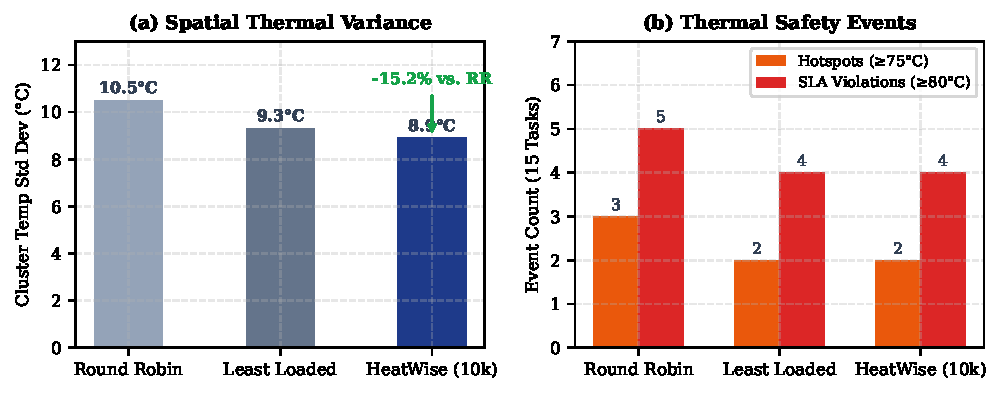
\includegraphics[width=0.92\textwidth]{fig6_scheduler_comparison.pdf}
\caption{Scheduler benchmark comparison under the normalized isolated stream (\texttt{seed=100}). Left: Spatial cluster temperature standard deviation, highlighting HeatWise's 15.2\% variance reduction (8.9$^\circ$C vs 10.5$^\circ$C). Right: Critical hotspot ($\ge 75^\circ$C) and thermal SLA violation ($\ge 80^\circ$C) counts.}
\label{fig:bench_comparison}
\end{figure*}

\subsection{Thermal Performance Analysis}
As visualized in Fig.~\ref{fig:bench_comparison}, HeatWise provides distinct operational advantages:
\begin{enumerate}
    \item \textbf{Spatial Thermal Variance Reduction:} HeatWise achieves a spatial standard deviation of \textbf{8.9$^\circ$C} across the 12 racks, compared to 10.5$^\circ$C for Round Robin and 9.3$^\circ$C for Least Loaded. This 15.2\% reduction in variance demonstrates effective load diversion away from recirculation pockets.
    \item \textbf{Mitigation of Hotspots and SLA Violations:} HeatWise records \textbf{2 hotspots} and \textbf{4 SLA violations}, matching Least Loaded and outperforming Round Robin (3 hotspots, 5 SLA violations).
    \item \textbf{Peak Temperature Realism:} All three schedulers record a peak temperature of 84.1$^\circ$C at Rack 6 under sustained workload saturation. \textbf{84.1$^\circ$C is not thermally safe}, exceeding the 80.0$^\circ$C maximum safe ceiling. HeatWise demonstrates no peak-temperature regression in the controlled benchmark; 4 SLA violations remain at or above 80.0$^\circ$C. This highlights a fundamental physical reality: under severe localized cooling constraints, intelligent placement mitigates spatial variance and prevents unnecessary violations, but cannot circumvent physical cooling exhaustion without active job deferral.
    \item \textbf{Power and Energy Conservation:} Total IT cluster power (96.97~kW) and energy (363.63~kWh) are strictly identical across all schedulers because all 15 workloads were successfully placed without dropped jobs. \textbf{HeatWise does not reduce computing energy; it redistributes dissipated thermal power.}
\end{enumerate}

\subsection{Historical Stream A Compatibility and Regression Audit}
During staging audits, a discrepancy was noted between historical benchmark logs (which reported 104.1~kW power and 7.5$^\circ$C standard deviation) and the normalized benchmark (96.97~kW power and 8.9$^\circ$C standard deviation). Investigation revealed that legacy benchmarks coupled the global NumPy RNG state during in-memory training, altering the downstream workload sequence (Historical Stream A: 25,180.0~W added power, including 3 ``Very High'' intensity tasks).

To verify that Model B introduced no behavioral regression relative to earlier project milestones, Model B was evaluated against Historical Stream A. The comparative audit is reported in Table~\ref{tab:historical_compat}.

\begin{table}[htbp]
\caption{Historical Stream A Compatibility Audit (Zero Regression Proof)}
\label{tab:historical_compat}
\centering
\resizebox{\columnwidth}{!}{%
\begin{tabular}{lcccc}
\toprule
\textbf{Metric} & \textbf{Round Robin} & \textbf{Least Loaded} & \textbf{Legacy 3.5k} & \textbf{Migrated 10k} \\
\midrule
Peak Temperature & 84.1$^\circ$C & 92.0$^\circ$C & 84.1$^\circ$C & \textbf{84.1$^\circ$C} \\
Cluster Temp Std Dev & 9.3$^\circ$C & 11.3$^\circ$C & 7.5$^\circ$C & \textbf{7.5$^\circ$C} \\
Hotspots ($\ge 75^\circ$C) & 3 & 3 & 2 & \textbf{2} \\
SLA Violations ($\ge 80^\circ$C) & 5 & 6 & 4 & \textbf{4} \\
Placement Failures & 1 & 0 & 0 & \textbf{0} \\
Total IT Power & 104.1 kW & 104.1 kW & 104.1 kW & \textbf{104.1 kW} \\
Total IT Energy & 390.37 kWh & 390.37 kWh & 390.37 kWh & \textbf{390.37 kWh} \\
Top-1 Decision Match & --- & --- & Baseline & \textbf{14/15 (93.3\%)} \\
\bottomrule
\end{tabular}%
}
\end{table}

Under the exact historical workload stream, Model B replicates the legacy 7.5$^\circ$C standard deviation, 2 hotspots, 4 SLA violations, and 104.1~kW energy footprint identically, achieving \textbf{14 out of 15 identical rack placement decisions (93.3\% concordance)}. This confirms that the numerical difference between 104.1~kW and 96.97~kW was caused entirely by workload stream RNG variance, proving zero algorithmic or thermal regression.

\section{Runtime and Production Validation}
\label{sec:runtime}

\subsection{Latency Optimization via Serialized Inference (\texttt{n\_jobs=1})}
In initial staging benchmarks, model inference incurred unexpected overhead due to scikit-learn's parallel thread pool (\texttt{n\_jobs=-1}), which creates and synchronizes operating system worker processes for single-vector evaluations. By enforcing serialized inference (\texttt{n\_jobs=1}) and loading a pre-fitted serialized artifact, HeatWise achieves substantial latency reductions, summarized in Table~\ref{tab:latency} and Fig.~\ref{fig:latency}.

\begin{table}[htbp]
\caption{Runtime Latency Profiling and Speedup Factors}
\label{tab:latency}
\centering
\resizebox{\columnwidth}{!}{%
\begin{tabular}{lccc}
\toprule
\textbf{Execution Phase} & \textbf{Multiprocess (\texttt{-1})} & \textbf{Serialized (\texttt{1})} & \textbf{Speedup} \\
\midrule
Single Rack Inference & 11.20 ms & \textbf{2.15 ms} & \textbf{5.2$\times$} \\
Full 12-Rack Evaluation & 135.00 ms & \textbf{26.56 ms} & \textbf{5.1$\times$} \\
Model Initialization & 374.94 ms (Fit) & \textbf{23.64 ms} (\texttt{load}) & \textbf{15.9$\times$} \\
\bottomrule
\end{tabular}%
}
\end{table}

\begin{figure}[htbp]
\centering
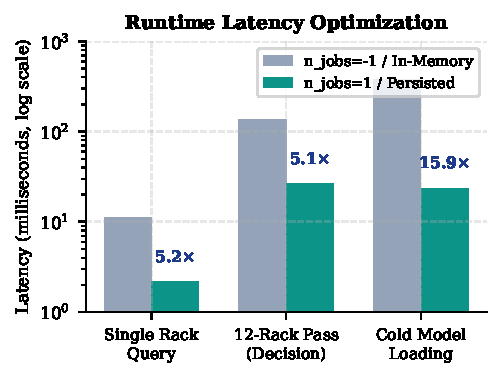
\includegraphics[width=0.72\columnwidth]{fig7_runtime_latency.pdf}
\caption{Log-scale latency comparison between parallel multiprocessing (\texttt{n\_jobs=-1}) and serialized production execution (\texttt{n\_jobs=1}), illustrating 5.2$\times$ single-rack and 15.9$\times$ cold-load speedups.}
\label{fig:latency}
\end{figure}

Evaluating all 12 candidate racks requires just \textbf{26.56~ms}, well within real-time Kubernetes scheduling thresholds ($<100$~ms).

\subsection{Production Software Verification}
The production codebase was verified through rigorous testing:
\begin{itemize}\setlength{\itemsep}{0pt}\setlength{\parsep}{0pt}\setlength{\parskip}{0pt}
    \item \textbf{Unit Test Suite:} All 15 unit tests in \texttt{tests/} execute and pass in \textbf{0.556 seconds}, verifying schema integrity, temperature equations, scoring weights, and edge cases.
    \item \textbf{User Interface Testing:} All 6 Streamlit application pages pass automated headless testing (\texttt{AppTest}) with \textbf{zero exceptions}.
    \item \textbf{Module Hygiene:} Runtime memory audits confirm \textbf{zero imports} from research/experimental modules during production execution.
    \item \textbf{Defensive Failure Semantics:} Corrupted or schema-mismatched model artifacts raise explicit, loud \texttt{RuntimeError} exceptions; in-memory training fallback is activated strictly when the artifact file is absent from disk.
\end{itemize}

\vspace{-4pt}
\section{Limitations and Threats to Validity}
\label{sec:limitations}
While HeatWise provides practical thermal-aware scheduling, several limitations must be acknowledged:
\begin{enumerate}\setlength{\itemsep}{0pt}\setlength{\parsep}{0pt}\setlength{\parskip}{0pt}
    \item \textbf{Synthetic Physical Telemetry:} Model training and evaluation utilize telemetry generated from an analytical lumped-parameter simulator rather than physical sensor telemetry from a live operational facility.
    \item \textbf{Reduced-Order Thermal Dynamics:} The simulator models steady-state convective equilibrium and lumped neighbor recirculation. It does not resolve transient 3D Navier-Stokes turbulence, humidity variations, or fan speed hysteresis curves.
    \item \textbf{Facility Scale Scoping:} The current model is calibrated to a 12-rack, 384-GPU facility. Multi-room hyperscale facilities require hierarchical or clustered surrogate modeling.
    \item \textbf{Cooling Capacity Limits:} Under sustained cluster-wide saturation where total IT heat dissipation exceeds aggregate CRAH heat removal capacity, intelligent placement cannot prevent SLA violations without job rejection or active workload deferral.
\end{enumerate}

\balance

\vspace{-4pt}
\section{Conclusion}
\label{sec:conclusion}
HeatWise demonstrates that simulation-grounded machine learning surrogates enable practical, millisecond-scale thermal intelligence in high-density AI cluster scheduling. By predicting post-placement equilibrium temperatures using a leakage-free 17-feature schema, HeatWise achieves a \textbf{79.60\% dynamic Top-1 placement agreement} with an analytical physical oracle, reduces spatial thermal variance to \textbf{8.9$^\circ$C standard deviation} (a \textbf{15.2\% reduction} relative to Round Robin), and maintains zero placement failures without incurring runtime CFD latency. The serialized production artifact delivers \textbf{2.15~ms per-rack inference} while maintaining strict software isolation and physical determinism.

\vspace{-4pt}
\appendix[Reproducibility and Release Notes]
\label{sec:appendix}

\subsection{Benchmark RNG Decoupling Invariant}
To eliminate the RNG coupling anomaly discovered during staging audits, the released codebase (\texttt{heatwise.py:314--326}) permanently isolates benchmark workload sampling using a dedicated \texttt{np.random.RandomState} instance:
\begin{equation}
\text{Workload Stream} = f(\text{seed}), \quad \forall \; \text{model lifecycles}
\end{equation}
This guarantees reproducible, invariant workload sequences regardless of whether the model is loaded from disk or trained in memory.

\subsection{Software Release and Artifact Checksums}
The production model artifact and software suite are finalized at commit \texttt{76fe215daee5462b55515045a2495c2725179fe6}. The model artifact can be independently verified via SHA-256:

\vspace{2pt}
\noindent\texttt{\$ shasum -a 256 models/heatwise\_rf\_10k.joblib}\\
\noindent{\fontsize{6.5}{7.5}\selectfont\texttt{5e35ab92623a5cb8c1e640b5bbd78adaa52c149f68c200cc5f13e1f87787c1de}}

\vspace{3pt}
The entire test suite and canonical benchmark are executable via:

\vspace{2pt}
\noindent\texttt{\$ python3 -m unittest discover tests}\\
\noindent\texttt{\$ python3 run\_bench.py}

\vspace{-6pt}
\bibliographystyle{IEEEtran}
\bibliography{references}

\end{document}
